\chapter{Implementation}
\label{chap:implementation}

This chapter presents an in-depth description of how \f{} works
and demonstrates how much it can simplify developers' experience
by showing real-world examples with extensive usage of its features.
Furthermore, since we are creating an open-source project, the structure of
the repository will also be analyzed.


\section{Overview}

\f{} is a transpiler which enhances serverless programming by introducing the concept of annotations.
Annotations are an abstraction layer that the developers can unobtrusively use
to apply code transformations and metadata generation to a given application,
which will be deployed to a serverless platform.

To achieve this goal, we used the \textit{TypeScript}\cite{ts} compiler API which lets us
manipulate sources with ease, and \textit{SLS}\cite{sls} which
uses the generated metadata to deploy to \textit{AWS Lambda}.

\begin{figure}[H]
  \centering
  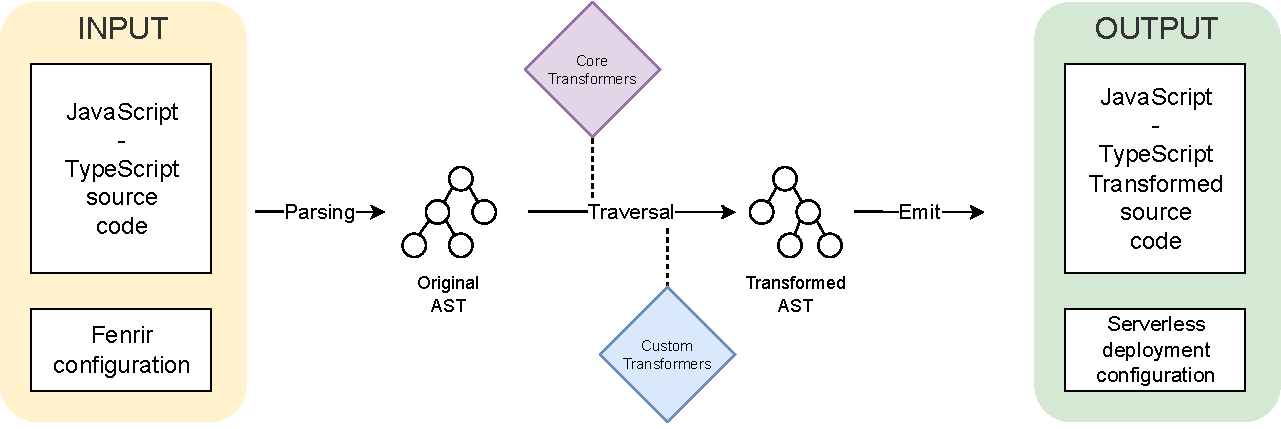
\includegraphics[width=\textwidth]{diagrams/pipeline}
  \caption{Transpiler pipeline.}
  \label{fig:pipeline}
\end{figure}

The transpilation pipeline, depicted in Figure \ref{fig:pipeline},
starts with the parsing of the input source code, which produces AST nodes with their related
annotations. Then, each annotation induces the application of its related
transformation step, whose output is fed into the next transformer, if any.
During the transformation steps, \f{} reports possible errors by gracefully
stopping the compilation process and indicating the offending instructions. Once
the transformations have taken place without any errors, the output code is saved
and the related metadata is also appended to a
\verb|serverless.yml| file which specifies function deployment
properties (e.g., the address to invoke a given function).

It is important to notice that \f{} doesn't lock developers in managing their
functions only through its tools, instead, its primary objective is to facilitate
the incremental adoption of the serverless paradigm.

% \subsection{Brief example: Monolith to Serverless conversion}

% Lorem ipsum dolor sit amet, qui minim labore adipisicing minim sint cillum sint consectetur cupidatat.

% \section{Detailed review}

% This section explains each step of the pipeline, defines annotations precisely and shows how to create new ones.

\section{Parsing}

\f{} requires a configuration file that must be named \verb|fenrir.config.json| to understand where to operate:

\begin{lstlisting}[language=json, caption={\f{} configuration}]
{
  "files": ["input/source.ts"],
  "serverlessConfigPath": "input/serverless.yml",
  "outputDirectory": "output",
  "annotations": {
    "CustomAnnotation": "annotations/custom-annotation.ts"
  }
}
\end{lstlisting}

The \verb|files| field accepts an array of filenames or a directory,
and it is used to represent which files will be parsed by the transpiler.

The \verb|serverlessConfigPath| field points at the input \textit{SLS} configuration
that must contain some mandatory input metadata, such as the region which the functions will be deployed on.

The \verb|outputDirectory| field indicates where the emitted files will be placed.

The \verb|annotations| field locates custom annotations as it takes an object
where the keys represent the new names and the values refer to their associated implementations.

\paragraph{\textbf{Fenrir's CLI}}
After creating the configuration, \f{} can be started through our CLI tool
by optionally passing as a flag the directory in which it is contained.
\begin{lstlisting}[language=bash, style=bashstyle]
# defaults to the current directory (.) for its file lookup...
> fenrir
# ...or uses a custom path
> fenrir -g input-directory
\end{lstlisting}
Furthermore, the CLI offers the \verb|init| sub-command to ease the setup needed for the entire pipeline
by generating the necessary boilerplate and configuration files.

% TODO: ricorda di parlare di quanto sia ottimo il compiler api di ts in Background.
% perché ha informazioni su tutto il progetto e non solo sui file.
\subsubsection{AST Traversal}

Through the \textit{TypeScript} compiler API, each sources' AST is traversed
by a visitor function which collects some data (e.g., dependencies imports) and examines
certain types of node in order to process annotations, namely \textit{exported function declarations}.
Lookups are restricted only to this syntactic category for two reasons:
\begin{itemize}
  \item \verb|export| ensures the functions are public and ready to be deployed.
  \item \verb|function declarations| minimize the code needed to control the AST.
    Considering that \textit{JavaScript} provides three distinct ways of declaring a function,
    accommodating all of these variations would inevitably result in a threefold expansion of the manipulation code.
    Moreover, function declarations are the idiomatic technique to write top-level functions.
\end{itemize}

\begin{lstlisting}[language=javascript, caption={Examples of processed or skipped nodes.}]
// Skipped
const a = 2;
// Skipped
for (const b of [1, 2, 3]) {}
// Processed
export function foo() {}
// Skipped
export const fiz = () => {}
// Skipped
export const bar = function() {}
\end{lstlisting}

The processed functions have their annotations examined, and
their bodies are visited to handle AST transformations.

\section{Annotations}

Annotations are syntactical units, or keywords, enclosed within JSDoc comments,
each associated with their respective transformer.
They can be expressed using a BNF-like syntax:
\begin{equation*}
\begin{aligned}
    \text{Annotation} & ::= "\$" \langle \text{Name} \rangle [ "(" \langle \text{Parameters} \rangle ")" ] \\
    \text{Name} & ::= [\text{a-zA-Z\_}][\text{a-zA-Z0-9\_}]* \\
    \text{Parameters} & ::= \langle \text{TypeScriptObject} \rangle \\
    \text{TypeScriptObject} & ::= \dots \\
\end{aligned}
\end{equation*}
This representation does not intend to provide a formal and precise depiction of the syntax of annotations.
Nevertheless, it serves to offer a general impression of how they can be written within the code.
\begin{lstlisting}[language=javascript, caption={Generic examples of annotation.}, label={lst:annotations-examples}]
/** $\dollar$Foo */

/** $\dollar$Bar(param: "first") */

/** $\dollar$Fiz(first: true, second: [1, 2, 3], third: (a, b) => a + b) */

/**
 * Annotations enrich docs...
 * $\dollar$Foo
 * ...and can even be multiline.
 * $\dollar$Bar(
 *    param: "fiz"
 * )
 *
 * all these explanatory texts are not 
 * harmful, as they are simply ignored.
 */
\end{lstlisting}

Annotations are designed to avoid cluttering \textit{JavaScript} with new syntax,
as they can only be written inside JSDoc comments.
Thus, they serve a dual-purpose by not only providing functionality
but also serving as supplementary documentation for the codebase.

Listing \ref{lst:annotations-examples} provides a valuable insight on how annotations
may be parameterized to modify transformers' functionality.
In fact, arguments undergo parsing as a \textit{TypeScript} object literal,
hence, they are as powerful as regular objects\cite{mdn_objects}
meaning that even complex structures (arrays, functions, etc...) can be used
during the compilation step to enrich transformations.

Another crucial feature of annotations is their composability,
as multiple annotations can be written within the same JSDoc,
essentially defining dedicated compilation pipelines by passing the output
of a transformation as input for the subsequent ones:
to facilitate this process, each source file may be visited multiple times.

\subsection{Core Annotations}

\f{} offers four core annotations whose transformers can handle code manipulation,
deployment metadata, or a combination of both functionalities:
by pipelining annotations, we can effectively utilize the strengths of different approaches.

\begin{table}[htbp]
    \centering
    \caption{Core annotations}
    \begin{tabular}{llcc}
        \toprule
        \textbf{Name} & \textbf{Code} & \textbf{Metadata} \\
        \midrule
        \$Fixed & Yes & Yes \\
        \$TrackMetrics & Yes & No \\
        \$HttpApi & No & Yes \\
        \$Scheduled & No & Yes \\
        \bottomrule
    \end{tabular}
\end{table}

\subsubsection{\$Fixed}
\annotation{\$Fixed(memorySize?: number, timeout?: number, ...)}
converts monolithic functions into \textbf{fixed}-size serverless functions,
whose resources are statically determined and remain constant regardless of the workload or input size.
To achieve this conversion, code is handled as follows:
\begin{itemize}
  \item The monolithic functions' parameters are mapped to a single \verb|event|
    parameter in order to adhere to \textit{AWS Lambda} serverless functions' signature.
  \item The monolithic functions' return statements change to match
    the shape of the response expected by the platform,
    by creating an object with a status code (\verb|200|)
    and a body that contains a serialized version of the initially returned value.
  \item Early return statements and throw statements are modified similarly,
    but the status code represents a client error (\verb|400|).
\end{itemize}

\annotation{\$Fixed} has no mandatory parameters, however, all the specified arguments will be
passed as metadata for the function deployment.

% ----------------------------------------------------------
% FIXED EXAMPLE
% ----------------------------------------------------------
\begin{lstlisting}[language=javascript, caption={Input code for \annotation{$\dollar$Fixed}}]
/** $\dollar$Fixed(timeout: 10) */
export async function foo(id) {
  if (!isValid(id)) {
    throw new Error('Something went wrong')
  }

  const data = await query()

  return data
}
\end{lstlisting}


\begin{lstlisting}[language=javascript, caption={Output code from \annotation{$\dollar$Fixed}}]
/** $\dollar$Fixed(timeout: 10) */
export async function foo(event) {
  const id = event.id

  if (!isValid(id)) {
    return {
      statusCode: 400,
      body: JSON.stringify({
        error: "'Something went wrong'",
      }),
    }
  }

  const data = await query()

  return {
    statusCode: 200,
    body: JSON.stringify(data),
  }
}
\end{lstlisting}

\begin{lstlisting}[language=yaml, caption={Generated Metadata through \annotation{$\dollar$Fixed}}]
functions:
  foo:
    handler: output/source.foo
  timeout: 10 # default is 6 seconds
\end{lstlisting}
% ----------------------------------------------------------
% FIXED EXAMPLE
% ----------------------------------------------------------

\subsubsection{\$TrackMetrics}
\annotation{\$TrackMetrics(namespace: string, metricName: string, metricValue?: ts.Expression)}
generates code that monitors and logs the functions’ resource usage
by also importing the necessary dependencies, i.e., for \textit{AWS Lambda}
it uses and injects the \textit{CloudWatch} dependency.
These are the required properties:
\begin{itemize}
  \item The function declaration must be \verb|async|.
    Preceding this annotation with \annotation{\$Fixed} makes it automatically \verb|async|.
  \item \verb|namespace| and \verb|metricName| are mandatory strings.
    The former represents the namespace instantiated on the cloud through \textit{AWS}.
  \item The third parameter, if present, must be the same as one of the variables' identifiers.
\end{itemize}

An example should be more explicative:
% ----------------------------------------------------------
% TRACK EXAMPLE
% ----------------------------------------------------------
\begin{lstlisting}[language=javascript, caption={Input code for \annotation{$\dollar$TrackMetrics}}]
import { query } from '../local'

/**
 * $\dollar$TrackMetrics(namespace: 'shop', metricName: 'sell', metricValue: size)
 */
export async function processOrder(id) {
  const order = await query(id)
  const size = order.size
  // ...more logic...
  return size
}
\end{lstlisting}


\begin{lstlisting}[language=javascript, caption={Output code from \annotation{$\dollar$TrackMetrics}}, label={lst:out-track}]
import { query } from '../local'
import { CloudWatch } from 'aws-sdk'

/**
 * $\dollar$TrackMetrics(namespace: 'shop', metricName: 'sell', metricValue: size)
 */
export async function processOrder(id) {
  const order = await query(id)
  const size = order.size
  await new CloudWatch()
    .putMetricData({
      Namespace: 'shop',
      MetricData: [
        {
          MetricName: 'sell',
          Timestamp: new Date(),
          Value: size,
        },
      ],
    })
    .promise()
  // ...more logic...
  return size
}
\end{lstlisting}
% ----------------------------------------------------------
% TRACK EXAMPLE
% ----------------------------------------------------------

Listing \ref{lst:out-track} shows the generated boilerplate to enable logs inside the function,
and an additional import statement is included at the top of the file to address its previous absence.
\annotation{\$TrackMetrics} puts the code in a context-aware manner,
placing it after the variable declared as \verb|metricValue|.

Supposing a typographical error was written instead of \verb|size|, the following error message would appear:
\begin{lstlisting}[language=console]
'$\dollar$TrackMetrics' can only receive an identifier as
a value for the 'metricValue' parameter like
'id' | 'order' | 'size'
in function 'processOrder' defined here:
--> input/source.ts:6
\end{lstlisting}

\subsubsection{\$HttpApi}
\annotation{\$HttpApi(method: string, path: string, ...)}
generates the metadata needed to make the function available as an HTTP endpoint.
\begin{itemize}
  \item The \verb|method| parameter represents the desired HTTP method (\verb|GET|, \verb|POST|, etc...).
  \item The \verb|path| parameter represents the URL path where the function will be available.
  \item The optional parameters are meant to customize the behavior of the HTTP endpoint further,
     for example, by setting up Cross-Origin Resource Sharing (CORS) headers.
\end{itemize}
% ----------------------------------------------------------
% Http EXAMPLE
% ----------------------------------------------------------
\begin{multicols}{2}[\columnsep=1cm]
\begin{lstlisting}[language=javascript]
/**
 * $\dollar$HttpApi(method: "POST", path: "/users/create")
 * $\dollar$HttpApi(method: "PUT", path: "/users/update")
 */
export function foo() {}
\end{lstlisting}

\columnbreak

\begin{lstlisting}[language=yaml]
foo:
  handler: output/source.foo
  events:
    - httpApi:
        method: POST
        path: /users/create
    - httpApi:
        method: PUT
        path: /users/update
\end{lstlisting}
\end{multicols}
% ----------------------------------------------------------
% Http EXAMPLE
% ----------------------------------------------------------

\subsubsection{\$Scheduled}
\annotation{\$Scheduled(rate: string, ...)}
generates the metadata needed to make the function run at specific dates or periodic intervals.
\begin{itemize}
  \item The \verb|rate| parameter is a rate or cron expression
    which schedules when the function should be triggered.
  \item The optional parameters are meant to customize the behavior of the scheduled event further,
     for example, by specifying multiple schedule expressions and giving it a description.
\end{itemize}
% ----------------------------------------------------------
% Scheduled EXAMPLE
% ----------------------------------------------------------
\begin{multicols}{2}[\columnsep=2cm]
\begin{lstlisting}[language=javascript]
/**
 * $\dollar$Scheduled(rate: "rate(2 hours)")
 */
export function foo() {}
\end{lstlisting}
\columnbreak

\begin{lstlisting}[language=yaml]
foo:
  handler: output/source.foo
  events:
    - schedule:
        rate: rate(2 hours)
\end{lstlisting}
\end{multicols}
% ----------------------------------------------------------
% Scheduled EXAMPLE
% ----------------------------------------------------------

\subsection{Custom Annotations}

\f{} isn't bound to its core annotations, as it endorses the creation of new ones
to fit custom requirements and usages.

In order to inform \f{} on the new annotation name and its transformer implementation,
the configuration file (i.e., \verb|fernrir.config.json|) must be updated:
\begin{lstlisting}[language=json]
{
  ...
  "annotations": {
    "IoT": "annotations/iot-impl.ts"
  }
}
\end{lstlisting}

\f{} encourages strict type-safety by offering a type definition for custom transformers:
\begin{lstlisting}[language=javascript, caption={Custom transformer for a new \annotation{$\dollar$IoT} annotation.}, label={lst:custom-transformer}]
// in 'annotations/iot-impl.ts'
import type { CustomTransformer } from 'fenrir-core'

type IotTransfomer = CustomTransformer<'IoT', { sql: string }>

const transformer: IotTransfomer = (
  node,
  context,
  annotation
) => {
  // ...implementation...
}

// custom transformers must be exported as `default`
export default transformer
\end{lstlisting}

Analyzing custom transformers' signature also provides insights on how
core annotations are implemented, since their definitions are almost identical.

The \verb|node| argument represents the function declaration in the AST which was marked with the annotation.
It contains all the relevant information associated with this type of AST node,
including the function's body, name, parameters, and other relevant details.

The \verb|context| argument represents the \textit{TypeScript} transformation context,
which is a very powerful object containing:
\begin{itemize}
  \item Methods for source code manipulations, such as\\\verb|context.factory.updateIfStatement()|.
  \item The typechecker, which is an essential module integrated in \textit{TypeScript}, useful for working with symbols:
    it has access to every type of each node and details about the project dependencies.
  \item Miscellaneous methods to handle lexical environments and compiler options.
  \item \f{} utilities that facilitate the development of transformers and of metadata handling.
\end{itemize}

The \verb|annotation| argument is an object containing the annotation name
and a record of all the arguments passed to it.
Its type definition is inferred from the previously established \verb|CustomTransformer| schema.

A transformer's return type can be omitted as it is inferred, however,
if it is manifested to provide a stricter signature, it is restricted to this subset:
\begin{lstlisting}[language=javascript, numbers=none]
type TransformerReturnType =
  | ts.SourceFile
  | ts.FunctionDeclaration
  | undefined
  | void
\end{lstlisting}
Hence, transformers may perform three types of tasks:
modifying the entire source file, which is useful for updating import declarations,
altering the function itself,
or solely modifying the metadata without changing the source code.

\section{Emit}

Magari parlare della gestione degli errori. E poi dell'emit.
E di come gli argomenti sono trattati.
